\chapter{Umsetzung} %Should be roughly 18pages
\label{kap:umsetzung}
\minitoc\pagebreak
% Erst JIRA Stories dann Datenmodell oder andersrum?
% Benötigtes Modell, dann stories, dann umsetzung
% Added new Data models like cpr, shocks, nibp!! as subsections!
% Viele Sachen Parallel...

\section{Technische Aspekte}
\label{sec:tech}
Zu Beginn der Umsetzung gilt es vorab diverse technische Aspekte zu analysieren und im Laufe der Entwicklung zu berücksichtigen.
Hierzu gehören beispielsweise die Schnittstelle und der daraus resultierende Export der Daten oder die Haltung der Daten in einer Datenbank.
Dies ist eine essentielle Basis, damit eine effiziente und angemessene Datengrundlage für die anschließend entwickelten Dashboards und Auswertungen zur Verfügung steht.

Dabei ist es bezüglich der Flexibilität und Unabhängigkeit von Vorteil , dass die Daten und der entsprechende Export nicht ausschließlich für die hier verwendete Technologie Qlik Sense abgestimmt und entwickelt werden.
Auch andere Software-Lösungen, Drittanbieterprogramme oder Business-Intelligence-Werkzeuge sollen die Daten und den neuen Export von \gls{ANALYSE} zur Auswertung verwenden können, damit eine gewisse Freiheit und keine absolute Abhängigkeit an einer Technologie entsteht.

\subsection{Schnittstelle \acrlong*{ANALYSE} und Qlik Sense} %StandDerTechnik??
\label{sub:schnittstelle}
Qlik Sense bietet eine Reihe an möglichen Datenverbindungen oder sogenannten \glqq Konnektoren\grqq.
Diese sind je nach Verbindungstyp vorgefertigte Module, welche die Verbindung zu gängigen Datenbanken oder anderen Quellen vereinfachen sollen.
Es können Daten aus lokalen Dateien wie CSV-, Excel- oder XML-Dateien, Datenbanken oder mittels standardisierten Schnittstellen geladen werden.
\bildbreit
{konnektoren}
{Qlik-Konnektoren zur Einrichtung von Datenverbindungen zu Datenbanken oder Schnittstellen}
{Qlik-Konnektoren für Datenverbindungen }

In Abbildung \ref{fig:konnektoren} sind die möglichen Datenbank- oder Schnittstellen-Konnektoren aufgelistet, wie beispielsweise \glqq MongoDB\grqq, \glqq Oracle\grqq, \glqq Microsoft SQL Server\grqq{} oder \glqq REST\grqq.

Da (wie in \ref{sub:StandTEchnikAnalyse} beschrieben) hinter \gls{ANALYSE} eine MongoDB-Datenbank steht, wäre der entsprechende Konnektor eine Möglichkeit, um die Einsatzdaten in Qlik bereitzustellen.
Allerdings befindet sich dieser zum einen in einem Beta-Zustand, zum anderen widerspricht dies der Philosophie, einen universellen Export der Daten zu bieten, da nicht jede Technologie einen Konnektor zur MongoDB hat. 

Ein weiterer Faktor ist außerdem die Sicherheit der Daten.
Gewährt man einem Drittprogramm und damit mehreren Nutzern den direkten Zugriff auf eine Datenbank, entstehen gewisse Risikofaktoren, welche die Sicherheit des Systems gefährden.
Schließlich liegen gegebenenfalls personenbezogene Daten in der Datenbank \ref{sec:rechtlich} oder Daten, welche gewisse Entscheidungen zur Folge haben.
Eine mögliche unkontrollierte Manipulation dieser Information sollte vermieden werden.

Demnach sollte es eine Schnittstelle von \gls{ANALYSE} geben, welche die Daten kontrolliert bereitstellt.
Eine sehr geeignete Technologie hierfür ist eine \gls{REST}ful API.
Vorteile hiervon sind laut Steimle \cite[2.3]{Steimle.2014} und Tilkov \cite[1.1]{Tilkov.2011} unter anderem:
\begin{itemize}
\item Die Kopplung der Systeme wird so gering wie möglich gehalten. 
Durch die homogen entwickelte Schnittstelle sind alle möglichen Vorgänge definiert und deren Aufruf spezifiziert.
So werden ungewollte Zugriffe auf die Daten in der Datenbank vermieden
\item Die gewollte Interoperabilität wird stark gewährleistet, da \gls{REST} auf gängigste Standards setzt. 
Dadurch können die meisten derzeitigen und zukünftigen Systeme mit dieser Technologie kommunizieren.
\item Die Wiederverwendung ist durch die einmalige Definition der Schnittstelle sehr hoch.
\item Die Skalierbarkeit und die daraus resultierende Performance kann mit \gls{REST} auch bei häufigen und großen Anfragen gewährleistet werden.
\end{itemize}

Außerdem bietet \gls{REST} die Möglichkeit, Zugriffe nur mit einer Authentifizierung durchzuführen.
Dies spiegelt das derzeitige Benutzergruppen-Konzept von den \cweb-Produkten sehr gut wider.

Mit diesen auf die Anforderungen passenden Vorteilen wurde sich für eine Schnittstelle der \gls{REST}-Technologie entschieden.
\gls{ANALYSE} besitzt bereits ein \gls{REST}-Interface, allerdings hat dieses bis dato einen anderen Zweck.

\subsection{Export der Daten} %subsub?
\label{sub:export}
Nach Festlegung der Technologie für die zukünftige Schnittstelle in \ref{sub:schnittstelle} werden nun die weiterführenden Schritte geplant und umgesetzt.
Das bestehende \gls{REST}-Interface soll demnach um einen Endpoint erweitert werden, welcher die Daten, respektive die \gls{MM} von allen Einsätzen eines \gls{ANALYSE}-Servers exportiert.

Dabei soll von Vornherein eine Authentifizierung notwendig sein, um die entsprechenden Daten des Servers zu erhalten.
Hierfür wird zunächst das \glqq Baisc Authentication\grqq-Verfahren als HTTP-Authentifizierung verwendet. 
Dabei können die angelegten Benutzer im aktuellen Mandanten von \gls{ANALYSE} sich mit dem entsprechenden Passwort im Header des \gls{REST}-Calls authentifizieren.

\subsubsection{Erstes Exportformat}
\label{subsub:1stexport}
Der erste Ansatz für einen solchen Export war ein zweistufiger Prozess:
\begin{enumerate}
\item Ein Export wird angestoßen, welcher von allen vorhandenen Einsätzen die jeweilige \gls{UUID} im Response-Body zurückgibt.
\end{enumerate}

Dieser erste Schritt wird mit der HTTP-Methode \glqq GET\grqq{} ausgeführt.
Im Header der Anfrage ist die in \ref{sub:export} genannte Authentifizierung sowie das entsprechende Format der Anfrage, der \glqq content-type\grqq, festgelegt.

Als Parameter können außerdem die maximale Anzahl an UUIDs sowie eine \gls{CQL}-Abfrage mitgegeben werden.
Ein Beispiel eines solchen Befehls kann dabei so aussehen:

\code{-GET http://corpsrv5009:8080/v3/missionlist/missions/query/start?cql=hasShocks\& batchsize=2000}
Code oder Bild (mit Zahlen)?

Mit diesem Befehl werden beispielsweise alle UUIDs der Einsätze geladen, die mindestens eine Defibrillation vorzeigen. 
Mittels des Parameters \glqq batchsize\grqq{} wird die Antwort auf maximal 2000 Einsätze beschränkt.
Das zurückgelieferte Objekt ist dabei ein JSON-Objekt mit einem Key-Value-Paar \code{"'uuids"': []}, welches als Wert die vielen \gls{UUID}s in einem Array speichert.

\begin{enumerate}[resume]
\item Im zweiten Schritt werden mit den erhaltenen UUIDs die weiterführenden \gls{MM} der Einsätze angefordert.
\end{enumerate}

Im Gegensatz zum ersten Schritt wird hierbei die HTTP-Methode \glqq POST\grqq{} verwendet.
Dies hat den Hintergrund, dass so die möglicherweise enorme Anzahl an \gls{UUID}s in den Request-Body des Befehls geschrieben werden können, statt in die URL.
Demnach wird der Body der Anfrage mit dem zuvor erhaltenen JSON-Objekt, sowie den gewünschten \gls{MM} beschrieben.
Auch hier ist wieder eine Basic-Authentifizierung notwendig, damit kein unerlaubter Zugriff auf die Daten erfolgen kann.\todo{Dark or White Theme?}

\begin{figure}[ht]
\begin{subfigure}{.5\linewidth}
  \centering
  % include first image
  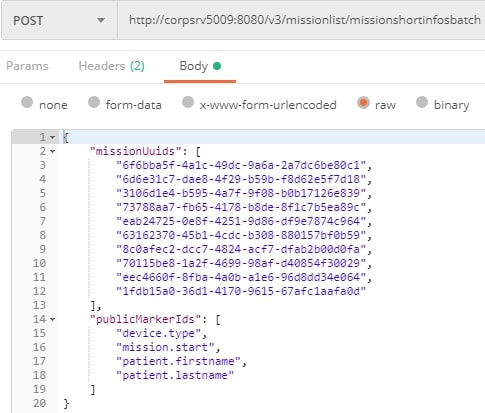
\includegraphics[width=.95\linewidth]{img/exRequestW}  
  \caption{Beispiel des POST-Requests}
  \label{fig:request}
\end{subfigure}
\begin{subfigure}{.5\linewidth}
  \centering
  % include second image
  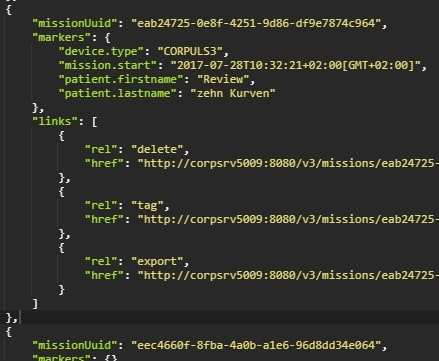
\includegraphics[width=.95\linewidth]{img/exResponse}  
  \caption{Auszug der Antwort auf den POST-Request}
  \label{fig:response}
\end{subfigure}
\caption[Beispiel einer Anfrage und Antwort der POST-Methode]{Beispiel einer Anfrage und Antwort der POST-Methode, um die \gls{MM} der im Body angegebenen Einsätze zu erhalten}
\label{fig:fig}
\end{figure}

In Abbildung \ref{fig:request} ist ein solcher POST-Request zu sehen.
In der URL wird der entsprechende \gls{ANALYSE}-Server adressiert, um auf die Daten der einzelnen Einsätze zugreifen zu können.
Im Body werden hierbei die aus Schritt 1 angeforderten Objekte eingefügt: \glqq missionUuids\grqq{} und \glqq publicMarkerIds\grqq.

Als Antwort erhält man mehrere \glqq Missions-Objekte\grqq{}, welche die \gls{UUID} und die entsprechenden \gls{MM} mit den individuellen Werten einer Mission enthält.
Ein Auszug einer solchen Antwort ist in \ref{fig:response} zu sehen.
Des Weiteren gibt es ein \glqq Link-Objekt\grqq{}, mit welchem ein Einsatz gelöscht, exportiert oder verändert werden kann. 

Positiv an diesem Export ist, dass die Anzahl der exportierten bedingt festgelegt werden kann.
Allerdings wird dieses Schema bei größeren Datenmengen, was genau das Ziel bei den Auswertungen ist, zu Problemen führen.
So kann das entsprechende Objekt mit den Einsatz-\gls{UUID}s sehr groß werden und beim kopieren und einfügen in den darauffolgenden Request-Body Schwierigkeiten bereiten.
Auch der damit resultierende große POST-Befehl ist keine optimale Umsetzung.

Aus diesem Anlass muss dieses Export-Format neu überdacht und für große Datenmengen optimiert werden.

\subsubsection{Überarbeitetes Export-Format}
\label{subsub:aktuellesformat}
Der Hauptaspekt beim neuen Entwurf der Export-Schnittstelle war das effiziente und sichere Umgehen mit großen Datenmengen.
Hierfür muss ein anderer als der zweistufige, in \ref{subsub:1stexport} beschriebene Prozess, entwickelt werden.

\todo{Lehmann fragen, welche anderen Alternativen Pläne es gab!}
\lipsum*[104]

Letztendlich wurde sich für ein/das Konzept mit den folgenden möglichen Schritten entschieden:
\begin{enumerate}
\item Die Generierung eines Exports anstoßen
\item Alle angeforderten Exports auflisten
	\begin{enumerate}
	\item Details zu einem explizitem Export bekommen
	\item Bestimmten Export löschen
	\end{enumerate}
\item Objekt/Datei mit allen Einsätzen und zugehörigen Daten mittels eigenem Link abrufen
\end{enumerate} 

Zum Erhalt der Export-Datei sind alle drei Schritte notwendig, 2a) \& b) sind als optionale Funktionen verfügbar.
Auch hier ist bei allen Vorgängen eine entsprechende Authentifizierung notwendig, um entsprechende Aktionen anzustoßen oder Informationen zu erhalten.

\begin{enumerate}
\item \code{-POST http://10.97.3.109:8080/v3/exports}
\end{enumerate}
Der erste Vorgang ist hierbei der POST-Befehl, der auf dem entsprechenden Server die Generierung eines neuen Exports anstößt.
Dabei werden alle verfügbaren Einsätze mit allen vorhandenen \gls{MM} exportiert.
Dies wurde so festgelegt, da der Anwender in der Regel mit einem solchen Export alle Missionen erhalten möchte.
Die Erweiterung um einen ressourcensparenden \glqq Incremental Load\grqq{} wird in \ref{sub:incremental} weiter betrachtet.

\begin{enumerate}[resume]
\item \code{-GET http://10.97.3.109:8080/v3/exports}
\end{enumerate}

Daraufhin ist es mit dem zweiten Schritt möglich, alle angestoßenen, laufenden und fertigen Exports aufzulisten.
Dabei wird mit der identischen URL die GET-Methode ausgeführt.
Hierbei werden pro Export zusätzliche Informationen bereitgestellt (siehe Abbildung \ref{fig:exportListWide}): 

%Die Start-Zeit (\glqq startTime\grqq) als UTC-Zeitstempel in Millisekunden, wann dieser Export angestoßen wurde.
%Analog der End-Zeitpunkt (\glqq endTime\grqq) wann dieser Export fertiggestellt wurde, die Anzahl Missionen, der jeweilige Status, ob angestoßen, laufend oder fertig, Links für weitere Optionen sowie die ID des Exports.

\begin{itemize}
\item Start-Zeit (\glqq startTime\grqq): UTC-Zeitstempel in ms, wann dieser Export angestoßen wurde
\item End-Zeit (\glqq endTime\grqq): UTC-Zeitstempel in ms, wann dieser Export fertiggestellt wurde
\item Anzahl der exportierten Einsätze (\glqq missions\grqq)
\item Status, ob angestoßen, laufend oder fertig
\item Links zu den weiteren Optionen
\item Die ID des Exports
\end{itemize}

\bild
{exportListWide}
{12cm}
{Antwort des Servers - Auszug der Auflistung von zwei fertiggestellten Exports als JSON-Objekte}
{Auflistung von Exports}

Demnach werden angeforderte Exports für eine ausgewählte Dauer gespeichert, was für unterschiedliche Szenarien ein Vorteil sein kann.
Auch die Möglichkeit, einen angeforderten Export wieder zu löschen ist eine hilfreiche Funktion, welche einen Server entlasten kann, sollten beispielsweise zu viele Exporte angefordert worden sein.
Der Status ist ebenfalls eine nützliche Information, welche den Empfang des fertigen Exports an ein \gls{BI}-Werkzeug erleichtern und garantieren kann.

\begin{enumerate}[resume]
\item \code{-GET http://10.97.3.109:8080/v3/exports/\{EXPORT\_ID\}/file}
\end{enumerate}

Im letzten Schritt wird der entsprechend bereitgestellte Link mitels GET-Methode aufgerufen.
Daraufhin erhält der Anwender den gesamten Export mit allen Einsätzen und den dazugehörigen \gls{MM} im JSON-Format. 
Ein Beispiel dieser Antwort ist Abbildung \ref{fig:exportFile} zu entnehmen.
\bild
{exportFile}
{9cm}
{Auszug des Exports mit allen Einsätzen und dazugehörige \gls{MM}}
{Auszug des Exports}

Der größte Vorteil dieses neuen Formats ist der Umgang mit großen Datenmengen.
Es müssen keine riesigen Objekte kopiert und eingefügt oder an eine andere Stelle weitergeleitet werden. 
Auch sind keine weiteren umständlichen Parameter notwendig. \\
Die URL wurde mit dem Schema \\
\colorbox[RGB]{240,240,240}{\texttt{http://\{SERVER\_IP\}/v3/exports}} \\
standardisiert, sodass keine unterschiedlichen URLs mit vielen optionalen Parametern wie in \ref{subsub:1stexport} notwendig sind.
Lediglich beim finalen Anfordern der Export-Datei muss die Standard-URL um \\
\colorbox[RGB]{240,240,240}{\texttt{http://\{SERVER\_IP\}/v3/exports\textcolor{red}{/\{EXPORT\_ID\}/file}}} \\
erweitert werden. 

\subsection{Erweiterung um tiefgreifendere? Daten}
\label{sub:erweiterung}
(json format cpr (siehe mails) (Fotos whiteboard als anhang?),)
null values bei cpr trends
%\subsection{Incremental Load?}
\subsubsection{Anforderungen an ein neues Export-Format (als User Stories in JIRA)}
\label{subsub:stories}

% Vor Export?
\subsection{Datenbankhaltung?}
\subsubsection{Lasttests?}
%dummydaten?
%\subsection{JIRA-Stories/Anforderungen als User Stories}

%\section{Datenmodell?}

\section{Erstellung der Qlik-App(s)}
\label{sec:erstellung}
%subsUnterschiedliche Apps?
\subsection{ETL-Prozess}
\label{sub:etl}

\subsubsection{Ladeskripte}
\label{subsub:scripts}

\subsubsection{Demo- und Testeinsätze herausfiltern}
\label{subsub:testfilter}

\subsubsection{Weitere manuell hinzugefügte Felder (ReaStart, Calendar, Test...)}
\label{subsub:weitereFelder}


\subsection{Datenmodell (hier oder eigene section?)}
\label{sub:datenmodell}

\subsection{Dimensionen}
\subsection{Kennzahlen}
\subsection{Verwendung von Erweiterungen?}
\subsection{Dashboards}
\subsubsection{Neue mögliche Visualisierungen durch Anforderungen Schocks, Nibp, Cpr}
test
\subsection{(Auszug) Umsetzung der Evaluierungsergebnisse}
\subsubsection{Zielgruppenunterschiedliche Startseiten}
\subsubsection{Lesezeichen?} %vlt so 10 Beispiel Lesezeichen
\subsubsection{Usability/Nutzerführung/Hilfetexte}
\subsubsection{Reduzierung Inhalt pro Arbeitsblatt}
\subsubsection{Weitere}
%subs testeinsätze filtern

\subsection{Einstellungen der Arbeitsblätter und Diagramme}
% (wie zB. Farben bei Auswahl beibehalten)
%CustomThemes?
%subs internationalisierung

% Aspekte vor Erstellung??
\section{Rechtliche Aspekte?}
\subsection{Datenschutz}
\subsection{Anonymisierung}


\section{Sonstige Aspekte?}
\subsection{Auslieferungsprozess?}
\subsection{Internationalisierung}
\subsection{Incremental Load?}
\label{sub:incremental}


\section{Evaluierung der Ergebnisse?}
%subs Usability-Tests?
